%\motto{Use the template \emph{chapter.tex} to style the various elements of your chapter content.}
\chapter{Grundlegende Quantenalgorithmen}
\label{basic_algorithms} % Always give a unique label
% use \chaptermark{}
% to alter or adjust the chapter heading in the running head

\chapterauthor{Vladimir Alyoshin, Gian-Luca Eberling}

\abstract*{some abstract}

\abstract{some abstract}

\section{Shor's Algorithmus zur Faktorisierung}

In der Informatik und insbesondere in der Kryptografie spielt die Sicherheit digitaler Kommunikation eine zentrale Rolle. Ein wesentliches Prinzip moderner Verschlüsselungsverfahren — etwa des RSA-Algorithmus — beruht auf der Annahme, dass die Zerlegung großer Zahlen in ihre Primfaktoren auf klassischen Computern mit exponentiellem Aufwand verbunden ist. Für ausreichend große Zahlen ist dieser Aufwand so gewaltig, dass selbst modernste Supercomputer über Jahre hinweg rechnen müssten, um einen privaten Schlüssel zu entschlüsseln.\\

Stellen wir uns vor, wir kennen lediglich eine große zusammengesetzte Zahl $N$, von der wir wissen, dass sie das Produkt zweier unbekannter Primzahlen $p$ und $q$ ist. Die klassische Faktorisierung würde in diesem Fall im schlimmsten Fall exponentiell viele Operationen erfordern. Genau hier setzt der Shor-Algorithmus an, der das Problem aus quantenmechanischer Sicht betrachtet.\\

Peter Shor entwickelte 1994 einen Algorithmus, der das Faktorisierungsproblem mithilfe eines Quantencomputers in polynomieller Zeit lösen kann — genauer gesagt in $\mathcal{O}((\log N)^3)$. Dies stellt eine exponentielle Beschleunigung gegenüber den besten bekannten klassischen Verfahren dar. Die zentrale Idee des Algorithmus liegt in der Reduktion des Faktorisierungsproblems auf das Periodenfindungsproblem, das sich durch Quanten-Phasenschätzung effizient lösen lässt.\\

Mit anderen Worten: Während klassische Computer für große $N$ praktisch keine Chance auf eine schnelle Faktorisierung haben, kann ein ausreichend großer Quantencomputer dieses Problem in überschaubarer Zeit lösen — mit drastischen Konsequenzen für die heute eingesetzten kryptografischen Verfahren.\\

Im Folgenden wird der Ablauf von Shors Algorithmus detailliert dargestellt und anhand eines konkreten Beispiels veranschaulicht. Dabei zeigen wir, wie Quantenregister, Quanten-Fourier-Transformation und die klassische Nachbearbeitung zusammenwirken, um die verborgenen Primfaktoren einer gegebenen Zahl zu enthüllen.\\


\subsection{Grundlagen: Primfaktorzerlegung und RSA}
Der RSA-Algorithmus basiert auf der Schwierigkeit, eine große Zahl \( N = pq \) zu faktorisieren. Shor’s Algorithmus bricht diese Sicherheit, indem er in polynomialer Zeit die Faktoren \( p \) und \( q \) bestimmt. Hat ein Angreifer Zugriff auf einen leistungsfähigen Quantencomputer, kann er aus dem öffentlichen Schlüssel die privaten Schlüsselparameter rekonstruieren. Shor's Algorithmus beschleunigt einen entscheidenen Schritt im klassischen Teil der Primfaktorzerlegung:

\begin{itemize}
  \item[a)] Wähle eine ganze Zahl \(x\) mit \(1 < x < N\).
  
  \item[b)] Berechne den größten gemeinsamen Teiler \(\gcd(x, N)\), z.\,B. mit dem Euklidischen Algorithmus.  
  \begin{itemize}
    \item Ist \(\gcd(x, N) \ne 1\), so gib \(\gcd(x, N)\) als nichttrivialen Teiler von \(N\) zurück und beende das Verfahren.
    \item Ist \(\gcd(x, N) = 1\), fahre mit Schritt c) fort.
  \end{itemize}
  
  \item[c)] Bestimme mit Hilfe des Quantenteils von Shor's Algorithmus die Ordnung \(r\) von \(x\) in der multiplikativen Gruppe \((\mathbb{Z}/N\mathbb{Z})^\times\), also das kleinste \(r \in \mathbb{N}\), sodass
  \[
  x^r \equiv 1 \mod N.
  \]
  
  \item[d)] Beginne erneut bei Schritt a), falls eine der folgenden Bedingungen zutrifft:
  \begin{itemize}
    \item \(r\) ist ungerade, oder
    \item \(x^{r/2} \equiv -1 \mod N\).
  \end{itemize}
  
  \item[e)] Berechne anschließend
  \[
  \gcd(x^{r/2} \pm 1, N)
  \]
  und gib mindestens einen der beiden Werte als nichttrivialen Teiler von \(N\) zurück.\\
  \[
  \]
  \textit{Hinweis:} Die so gefundenen Teiler müssen nicht direkt den gesuchten Primfaktoren \(p\) oder \(q\) entsprechen. Sie teilen jedoch \(N\) und können mit Hilfe des Euklidischen Algorithmus weiterverarbeitet werden, um auf die Primfaktoren zu schließen.
\end{itemize}


Shor's Algorithmus setzt bei Schritt c) ein und beschleunigt diesen massiv. Für einen klassischen Computer dauert es exponentiell lange diesen Schritt zu lösen. Dies zeigt, dass RSA bei hinreichend großen Quantencomputern als unsicher gelten muss.

Ziel ist es also, eine zusammengesetzte Zahl \( N = pq \) effizient zu faktorisieren. Um diese Faktorisierung zu beschleunigen nutzt Shor's Algorithmus die Periodizität der Funktion

\begin{definition}[Modulare Arithmetik] 
\[
f(a) = x^a \bmod N
\]
ist definiert als der Rest bei der Division von \(x^a\) durch \(N\).

\begin{itemize}
    \item \(x \in \mathbb{Z}\) ist eine Basiszahl, die kleiner als \(N\) und teilerfremd zu \(N\) sein sollte (d.h. \(\gcd(x, N) = 1\)).
    \item \(a \in \mathbb{N}_0\) ist der Exponent, eine natürliche Zahl (inkl. 0).
    \item \(N \in \mathbb{N}\) ist die zusammengesetzte Zahl, deren Primfaktorzerlegung wir bestimmen wollen.
    \item \(f(a)\) gibt den Rest an, wenn \(x^a\) durch \(N\) geteilt wird, also den Wert modulo \(N\).
\end{itemize}
\end{definition}
um mithilfe eines quantenmechanischen Verfahrens – konkret der Quanten-Phasenschätzung (QPE) – die Periode \( r \) dieser Funktion effizient zu bestimmen.

Im Algorithmus wird zunächst ein Superpositionszustand über viele Werte \( a \) erzeugt und anschließend durch eine unitäre Operation \( U_f \), die \( |a\rangle \mapsto |f(a)\rangle \) abbildet, mit den Funktionswerten moduliert.\\

Im nächsten Schritt erfolgt eine Quanten-Fouriertransformation (QFT) auf das Register, das die Werte von \( a \) enthält. Durch diese Fouriertransformation wird die Periodizität in der Amplitudenverteilung als charakteristische Spitzen (Peaks) sichtbar gemacht: Interferenzen zwischen den Zuständen führen dazu, dass bestimmte Frequenzanteile, die Vielfache von \( q/r \) (wobei \( q \) die Dimension des Registers ist) entsprechen, verstärkt werden, während andere ausgelöscht werden.\\

Je nach Konvention und Betrachtung kann man die QFT oder auch die inverse QFT (iQFT) verwenden; beide führen zur Hervorhebung der Periodizität im Zustandsraum, nur der genaue Ablauf der Transformation unterscheidet sich.\\

Nach der Fouriertransformation wird eine Messung durchgeführt, die mit hoher Wahrscheinlichkeit einen Wert \( c \) liefert, der näherungsweise in einem rationalen Verhältnis  
\[
\frac{c}{Q} \approx \frac{d}{r}
\]
zu \( r \) steht. Mithilfe der Kettenbruchentwicklung kann daraus die Periode \( r \) bestimmt werden.

Ist \( r \) bekannt und erfüllt sie bestimmte Voraussetzungen (z.B. \( r \) ist gerade und \( x^{r/2} \not\equiv -1 \bmod N \)), so lassen sich mit dem Euklidischen Algorithmus die Primfaktoren von \( N \) berechnen:  
\begin{definition}[Größter gemeinsamer Teiler (gcd)]
Der größte gemeinsame Teiler zweier Zahlen \(m, n \in \mathbb{N}\), bezeichnet als \(\gcd(m,n)\), ist die größte natürliche Zahl, die sowohl \(m\) als auch \(n\) ohne Rest teilt.\\

Im Kontext von Shor's Algorithmus verwenden wir
\[
\gcd\left(x^{r/2} \pm 1, N\right),
\]
wobei
\begin{itemize}
    \item \(x \in \mathbb{Z}\) eine Zahl ist, die teilerfremd zu \(N\) ist,
    \item \(r \in \mathbb{N}\) die Periode der Funktion \(f(a) = x^a \bmod N\) darstellt,
    \item \(N \in \mathbb{N}\) die zu faktorisierende zusammengesetzte Zahl ist,
    \item und \(x^{r/2} \pm 1\) eine Zahl ist, mit der wir durch die Berechnung des \(\gcd\) potenzielle Teiler von \(N\) finden.
\end{itemize}
\end{definition}

So nutzt Shor's Algorithmus die Quanteninterferenz und Fourier-Analyse, um versteckte Periodenstrukturen zu extrahieren und damit die Faktorisierung effizient zu ermöglichen.

\subsection{Aufbau des Shor Algorithmus}

Im folgenden Abschnitt werden wir alle notwendigen Methoden, Definitionen und Schritte beschreiben, die erforderlich sind, um den Shor-Algorithmus auszuführen. Dabei erklären wir Methode für Methode und wenden diese stets auf ein konkretes Beispiel an, um den Algorithmus möglichst präzise und anschaulich zu veranschaulichen. Anstelle einer sehr großen Zahl \( N \), wie sie in der Praxis als Schlüssel verwendet wird, wählen wir hier eine deutlich kleinere Zahl. \\

Der konkrete Fall, den wir betrachten, ist die Primfaktorzerlegung der Zahl \( N = 15 \). Natürlich kennen wir bereits die Primfaktoren \( 3 \) und \( 5 \). Es gilt somit \( N = q \cdot p \) mit \( q, p \in \mathbb{Z} \). \\

Zunächst muss festgelegt werden, wie groß der Hilbertraum \( Q = 2^n \) mit \( n \) Qubits sein muss, also die Gesamtanzahl aller Basiszustände des \( n \)-Qubit-Systems. Dies bestimmt, wie viele mögliche Zustände \( a \) betrachtet werden sollen. Dabei gilt die Bedingung
\[
2^n \geq N^2.
\]

Für unser Beispiel mit \( N = 15 \) ist \( N^2 = 225 \). Somit muss \( Q = 2^n \geq 225 \) gelten. Das entspricht mindestens \( n = 8 \) Qubits, da \( 2^8 = 256 \geq 225 \) ist. \\

Damit ergibt sich für das erste Register eine Größe von \( 8 \) Qubits. Das zweite Register benötigt
\[
m = \lceil \log_2(N) \rceil = \lceil \log_2(15) \rceil = 4
\]
Qubits.\\

Nun sind alle grundlegenden Variablen definiert und anhand eines konkreten Beispiels veranschaulicht. 
Bevor wir das Beispiel vollständig durchrechnen, formulieren wir zunächst die allgemeinen Schritte des Shor‑Algorithmus:

\begin{enumerate}
    \item \textbf{Initialisierung in einen Superpositionszustand:} 
    Die erste Operation besteht darin, zwei Quantenregister entsprechend der berechneten Qubit-Größen als Eingabe und Ausgaberegister zu erzeugen, welche sich alle in den Basiszuständen befinden, also mit der gleichen Wahrscheinlichkeit auftreten:
\[
\ket{\psi_0} = \ket{0}^{\otimes n} \otimes \ket{0}^{\otimes m}
\]
    Die \textit{Gleichverteilung} wird dadurch erreicht, dass die Amplituden aller Zustände gleich sind. Wenn das System anfangs im Zustand $\ket{0}^{\otimes n}$ ist (alle Qubits auf 0), dann erzeugen wir durch Anwendung der Hadamard-Transformation auf jedes Qubit die Superposition - aber nur auf das erste Register:

$$
\ket{\psi_1} = \frac{1}{\sqrt{Q}} \sum_{a=0}^{Q-1} \ket{a}
$$
Dabei ist:
  \begin{itemize}
    \item \( n \): Anzahl der Qubits im ersten Register.
    \item \( Q = 2^n \): Anzahl der möglichen Zustände im ersten Register
    \item \( x \): Laufvariable über alle Basiszustände von \( \ket{0} \) bis \( \ket{Q-1} \).
    \item \( 1 \): Anfangszustand des zweiten Registers, auf das später die modulare Exponentiation angewendet wird.
  \end{itemize}

  Durch die Hadamard-Gates wird das Register in eine Superposition gebracht, in der alle \( Q \) Basiszustände gleichwahrscheinlich sind. Diese Superposition ist notwendig, um später durch die Phaseninterferenz Information über die Periode der Funktion zu extrahieren.\\
 \item \textbf{Unitäre Funktion anwenden} 
\[
U_f \colon |a\rangle|1\rangle \mapsto |a\rangle|x^a \bmod N\rangle
\]
\begin{itemize}
    \item \textbf{\( a \)}: Wert im ersten Register (Index der Superposition), typischerweise \( a \in \{0, 1, \dotsc, Q-1\} \) mit \( Q = 2^n \), wobei \( n \) die Anzahl der Qubits im ersten Register ist.
    \item \textbf{\( x \)}: Eine zufällig gewählte ganze Zahl mit \( 1 < x < N \), die zu \( N \) teilerfremd ist.
    \item \textbf{\( N \)}: Die zusammengesetzte Zahl, deren Primfaktoren bestimmt werden sollen.
    \item \textbf{\( U_f \)}: Eine unitäre Transformation, die auf beiden Registern wirkt. Sie berechnet im zweiten Register die Funktion \( f(a) = x^a \bmod N \), wobei das erste Register \( |a\rangle \) als Steuerregister dient.
\end{itemize}

Nach Anwendung von \( U_f \) ergibt sich der verschränkte Zustand
\[
\ket{\psi_2} = \frac{1}{\sqrt{Q}} \sum_{a=0}^{Q-1} \ket{a} \otimes \ket{x^a \bmod N}
\]
Dieser Zustand ist eine Superposition über alle möglichen Paare \( (a, f(a)) \), wobei \( f(a) = x^a \bmod N \) die periodische Struktur trägt, die später durch die Quanten-Fourier-Transformation im ersten Register erkennbar gemacht wird.\\

\item \textbf{Quanten-Fourier-Transformation (QFT) auf das erste Register anwenden}

\noindent Die Quanten-Fourier-Transformation wird nun auf das erste Register angewendet. Diese transformiert den Zustand \( |a\rangle \) gemäß:

\[
\mathrm{QFT}(|a\rangle) = \frac{1}{\sqrt{Q}} \sum_{c=0}^{Q-1} e^{2\pi i \frac{a c}{Q}} |c\rangle
\]

\begin{itemize}
    \item \( Q = 2^n \): Anzahl der Basiszustände im ersten Register.
    \item \( a \): Index im ersten Register vor der QFT.
    \item \( c \): Index nach der Fouriertransformation – potenzieller Messwert.
\end{itemize}

\noindent Daraus ergibt sich der Gesamtzustand nach Anwendung der QFT:
\[
\ket{\psi_3} = \frac{1}{Q} \sum_{a=0}^{Q-1} \sum_{c=0}^{Q-1} e^{2\pi i \frac{a c}{Q}} \ket{c} \otimes \ket{x^a \bmod N}
\]

\noindent In der Quanten-Fourier-Transformation entsteht in jedem Summand der Ausdruck
\[
e^{2\pi i \frac{a c}{Q}},
\]
der eine komplexe \(Phasenrotation\) beschreibt.

\begin{itemize}
    \item \textbf{\( a \)}: Index des ursprünglichen Zustands im Superpositionsregister.
    \item \textbf{\( c \)}: Index des Zielzustands nach der Fouriertransformation.
    \item \textbf{\( Q \)}: Anzahl möglicher Zustände im Register (meist \( Q = 2^n \)).
\end{itemize}

\noindent Diese Phasenfaktoren lassen sich mit Hilfe der Euler-Formel interpretieren:
\[
e^{2\pi i \frac{a c}{Q}} = \cos\left(2\pi \frac{a c}{Q}\right) + i \cdot \sin\left(2\pi \frac{a c}{Q}\right)
\]

\noindent Es handelt sich also um eine \(Rotation\) \(im\) \(komplexen\) \(Raum\) – die komplexe Zahl liegt auf dem Einheitskreis und rotiert je nach Kombination von \( a \) und \( c \) um einen bestimmten Winkel. Dadurch ergibt sich:

\begin{itemize}
    \item Jeder Zustand \( |a\rangle \) trägt mit einer anderen Phase zur Superposition bei.
    \item Bei periodischer Struktur der Funktion \( f(a) = x^a \bmod N \) interferieren die komplexen Phasen systematisch.
    \item Dies führt dazu, dass bei der Messung des ersten Registers nur bestimmte Werte \( c \) mit hoher Wahrscheinlichkeit auftreten – die sogenannten \(Fourier-Peaks\).
    \item Andere Zustände löschen sich durch destruktive Interferenz aus.
\end{itemize}

\noindent Genau diese Interferenzstruktur erlaubt es, verborgene Perioden zu extrahieren – und damit den entscheidenden quantenmechanischen Vorteil zur Faktorisierung auszunutzen.\\

\item \textbf{Periodenbestimmung durch Kettenbruchentwicklung}

\noindent Nach der Fouriertransformation wird eine Messung durchgeführt, die mit hoher Wahrscheinlichkeit einen Wert \( c \) liefert, der näherungsweise in einem rationalen Verhältnis steht:
\[
\frac{c}{Q} \approx \frac{d}{r}
\]

\begin{itemize}
    \item \( c \): Messwert aus dem ersten Register nach Anwendung der QFT.
    \item \( Q \): Anzahl möglicher Zustände im ersten Register (typischerweise \( Q = 2^n \), mit \( Q > N^2 \)).
    \item \( d \): unbekannter ganzzahliger Zähler.
    \item \( r \): die Periode der Funktion \( f(a) = x^a \bmod N \), die bestimmt werden soll.
\end{itemize}

\noindent Ziel ist es, aus dem gemessenen Bruch \( \frac{c}{Q} \) eine möglichst genaue Näherung \( \frac{d}{r} \) zu finden, wobei \( r \) möglichst klein ist. Dies gelingt über die sogenannte \(Kettenbruchentwicklung\):

\begin{enumerate}
    \item Entwickle den Bruch \( \frac{c}{Q} \) in einen Kettenbruch.
    \item Brich die Entwicklung an mehreren Stellen ab und bilde die entsprechenden Konvergenten \( \frac{d_i}{r_i} \).
    \item Prüfe für jedes \( r_i \), ob \( x^{r_i} \equiv 1 \mod N \) gilt.
    \item Der kleinste passende \( r_i \) ist dann mit hoher Wahrscheinlichkeit die gesuchte Periode \( r \).
\end{enumerate}

\noindent Sobald die Periode \( r \) gefunden wurde, kann man im nächsten Schritt durch Berechnung des größten gemeinsamen Teilers (siehe \texttt{gcd}-Definition) mögliche Faktoren von \( N \) bestimmen:
\[
\gcd(x^{r/2} \pm 1, N)
\]

\noindent Damit ist der zentrale algorithmische Teil von Shor abgeschlossen – die restlichen Schritte sind rein klassisch.\\
\end{enumerate}

\noindent
Alle Operationen lassen sich im wesentlichen wie folgt zusammenfassen: Zunächst erfolgt die Initialisierung von zwei Quantenregistern, wobei das erste in eine Superposition aller möglichen Werte gebracht wird und das zweite den Ausgangszustand \( |1\rangle \) erhält. Durch Anwendung der unitären Funktion \( U_f \) wird eine Kopplung zwischen den Registern hergestellt, die die periodische Struktur der Funktion \( f(a) = x^a \bmod N \) abbildet. Anschließend findet die Quanten-Fourier-Transformation (QFT) auf dem ersten Register statt, wodurch mittels Interferenzinformation über die Periode \( r \) gewonnen wird. Die Messung des ersten Registers liefert eine Näherung an einen Bruch \( d/r \), aus dem mit der Kettenbruchentwicklung die Periode bestimmt wird. Auf Basis dieser Periode können die Teiler von \( N \) berechnet werden. \\

\noindent Die Operationen des Shor's Algorithmus zur Faktorisierung lassen sich wie folgt darstellen:

\begin{algorithm}[H] % <-- [H] erzwingt Platzierung an dieser Stelle
\caption{Shor's Algorithmus zur Faktorisierung einer Zahl \( N \)}
\label{algorithm:shor}
\begin{algorithmic}[1]
\Require Eine zusammengesetzte Zahl \( N \) aus zwei unbekannten Primzahlen \( p \) und \( q \)
\Ensure Ein nicht-trivialer Teiler von \( N \)
\State Wähle zufällig eine ganze Zahl \( x \) mit \( 1 < x < N \)
\If{\( \gcd(x, N) \neq 1 \)}
    \State \Return \( \gcd(x, N) \) \Comment{Zufällig gewähltes \( x \) war schon ein Teiler}
\EndIf
\State Bestimme die Periode \( r \) der Funktion \( f(x) = x^a \bmod N \) mittels Quanten-Phasenschätzung:
\State Initialisiere zwei Register: Eins mit Superposition aller \( x \), eins mit Zustand \( |1\rangle \)
\State Wende die unitäre Operation \( U_f \colon |a\rangle|1\rangle \mapsto |a\rangle|x^a \bmod N\rangle \) an
\State Wende die Quanten-Fourier-Transformation (QFT) auf das erste Register an
\State Miss das erste Register → erhalte Näherung \( d/r \)
\State Berechne \( r \) durch Kettenbruchentwicklung
\If{\( r \) ungerade oder \( x^{r/2} \equiv -1 \bmod N \)}
    \State \Return \textbf{Fehlschlag, wähle anderes \( a \)} und wiederhole
\EndIf
\State Berechne \( \gcd(x^{r/2} \pm 1, N) \)
\State \Return Einer der berechneten Teiler ist eine Primzahl \( p \) oder \( q \)
\end{algorithmic}
\end{algorithm}

\subsection{Rechenbeispiel – Shor's-Algorithmus}

Im folgenden Abschnitt wird das zu Beginn beschriebene Beispiel \( N = 15 \) vollständig durchgerechnet:

Wir wählen \( N = 15 \) und \( x = 2 \). Für den Algorithmus benötigen wir ein erstes Register mit mindestens \( n = 8 \) Qubits, sodass \( Q = 2^n = 256 > N^2 = 225 \) gilt. Das zweite Register benötigt nur \( m = \lceil \log_2 N \rceil = 4 \) Qubits, da es die Werte von \( f(a) = 2^a \bmod 15 \) aufnehmen muss.

\begin{enumerate}
    \item \textbf{Initialisierung in einen Superpositionszustand} \\
    Der Anfangszustand ist:

    \[
    \ket{\psi_0} = \ket{0}^{\otimes 8} \otimes \ket{0}^{\otimes 4}
    \]

    Nach Anwendung von Hadamard-Gattern auf alle 8 Qubits des ersten Registers entsteht die Gleichverteilung (Superposition) über alle \( Q = 256 \) Zustände:

    \[
    \ket{\psi_1} = \frac{1}{\sqrt{256}} \sum_{a=0}^{255} \ket{a} \otimes \ket{0}
    \]

    Diese Superposition ermöglicht es, alle Werte \( a \) gleichzeitig zu verarbeiten.\\

    \item \textbf{Anwendung der unitären Funktion \( U_f \)} \\

    Die Funktion \( f(a) = 2^a \bmod 15 \) wird auf das zweite Register angewandt, ohne das erste Register zu verändern. Die Transformation lautet:

    \[
    U_f: \ket{a} \ket{0} \mapsto \ket{a} \ket{2^a \bmod 15}
    \]

    Der Zustand nach Anwendung von \( U_f \) ist:

    \[
    \ket{\psi_2} = \frac{1}{\sqrt{256}} \sum_{a=0}^{255} \ket{a} \ket{2^a \bmod 15}
    \]

    Um das Verhalten der Funktion \( f(a) = 2^a \bmod 15 \) besser zu verstehen, berechnen wir die ersten Funktionswerte:

    \[
    \begin{array}{c|c}
    a & f(a) = 2^a \bmod 15 \\
    \hline
    0 & 1 \\
    1 & 2 \\
    2 & 4 \\
    3 & 8 \\
    4 & 1 \\
    5 & 2 \\
    6 & 4 \\
    7 & 8 \\
    8 & 1 \\
    \end{array}
    \]

    Wir erkennen: Die Funktionswerte wiederholen sich mit einer Periode \( r = 4 \), also \( 2^4 \bmod 15 = 1 \).
    \begin{figure}[H]
    \centering
    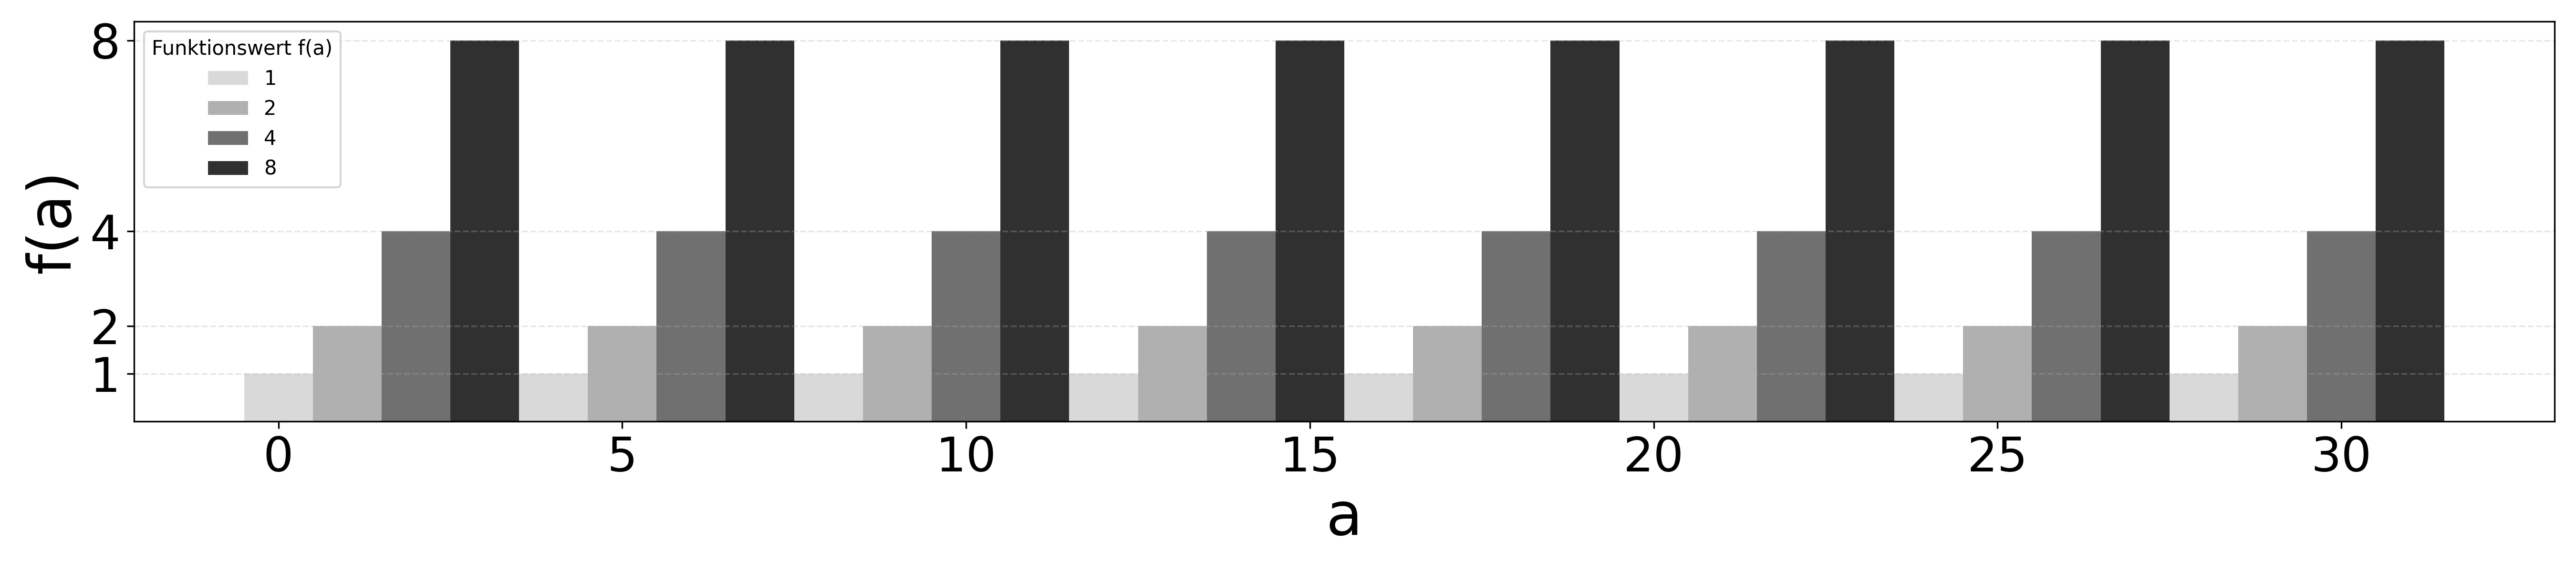
\includegraphics[width=1\textwidth,height=6cm,keepaspectratio]{images/basic-algorithms/shor_mod15_frequenz_graustufen.png}
    \caption{Visualisierung von $f(a) = 2^a \bmod 15$ mit Periode $r$ = 4}
    \label{fig:Visualisierung von $f(a) = 2^a \bmod 15$ mit Periode $r$ = 4}
\end{figure}

    Der verschränkte Zustand besteht also aus Gruppen gleicher Ausgabewerte:

    \[
    \ket{\psi_2} = \frac{1}{\sqrt{256}} \left( \ket{0} \ket{1} + \ket{4} \ket{1} + \ket{8} \ket{1} + \dots + \ket{252} \ket{1} + \dots \right) + \dots
    \]

    Dabei erscheinen alle \( a \)-Werte, die den gleichen Funktionswert liefern, gemeinsam mit dem jeweiligen \( \ket{f(a)} \).\\

    \item \textbf{Quanten-Fourier-Transformation (QFT)} \\

    Jetzt wenden wir auf das erste Register die QFT an. Die QFT transformiert die Basiszustände wie folgt:

    \[
    \mathrm{QFT}(\ket{a}) = \frac{1}{\sqrt{256}} \sum_{c=0}^{255} e^{2\pi i a c / 256} \ket{c}
    \]

    Die QFT wirkt linear auf jeden Summanden, sodass sich der Gesamtzustand ergibt als:

    \[
    \ket{\psi_3} = \frac{1}{256} \sum_{a=0}^{255} \sum_{c=0}^{255} e^{2\pi i a c / 256} \ket{c} \ket{2^a \bmod 15}
    \]

    Die Periode \( r = 4 \) der Funktion \( f(a) = 2^a \bmod 15 \) sorgt dafür, dass bei der Messung des ersten Registers besonders häufig Vielfache von \( \frac{Q}{r} = \frac{256}{4} = 64 \) auftreten. Erwartbare Messwerte sind also \( c \in \{0, 64, 128, 192\} \).\\

    \item \textbf{Messung und Kettenbruchentwicklung} \\

    Nehmen wir an, bei der Messung des ersten Registers erhalten wir \( c = 64 \). Daraus ergibt sich:

    \[
    \frac{c}{Q} = \frac{64}{256} = \frac{1}{4}
    \]

    Dies ist in diesem Beispiel bereits vollständig gekürzt – in der Praxis verläuft dies jedoch nicht immer so glatt. Über die Kettenbruchentwicklung von \( \frac{1}{4} \) folgt sofort \( r = 4 \) als vermutete Periode.\\

    \item \textbf{Faktoren berechnen} \\

    Mit der gefundenen Periode \( r = 4 \) testen wir, ob sich damit die Faktoren von \( N = 15 \) bestimmen lassen. Dafür prüfen wir:

\[
\gcd(x^{r/2} - 1, N) = \gcd(2^2 - 1, 15) = \gcd(3, 15) = 3
\]
\[
\gcd(x^{r/2} + 1, N) = \gcd(2^2 + 1, 15) = \gcd(5, 15) = 5
\]

    Wir erhalten die nicht-trivialen Faktoren 3 und 5 von \( N = 15 \). Die Faktorisierung ist damit erfolgreich abgeschlossen.\\

\textit{Hinweis:} Dass hier direkt beide Primfaktoren von \( N \) ermittelt werden, ist ein Glücksfall dieses kleinen Beispiels. In realistischen Anwendungen des Shor-Algorithmus ist es üblich, dass einer oder beide der berechneten Werte lediglich einen gemeinsamen Teiler mit dem ursprünglichen \( N \) ergeben. Diese Teiler führen aber dennoch – eventuell nach mehreren Wiederholungen von Euklids Algorithmus– zuverlässig zur vollständigen Faktorisierung, da der Algorithmus mit hoher Wahrscheinlichkeit mindestens einen nicht-trivialen Teiler liefert.

\end{enumerate}

Der Shor-Algorithmus zeigt, wie Quantencomputer periodische Strukturen in Funktionen aufdecken können, die klassisch nur mit exponentiellem Aufwand zu finden wären. Die Kombination aus Quanten-Phasenabschätzung, Fourier-Transformation und Kettenbruchentwicklung ermöglicht eine effiziente Faktorisierung großer Zahlen – ein fundamentaler Angriff auf die Sicherheit klassischer Verschlüsselung.\\

Damit stellt der Shor-Algorithmus einen Meilenstein in der Quanteninformatik dar: Er demonstriert das Potenzial quantenmechanischer Algorithmen, bestimmte Probleme deutlich schneller zu lösen als klassische Verfahren. Besonders betroffen ist dabei die auf der Faktorisierung großer Zahlen basierende Kryptographie, wie etwa RSA, deren Sicherheitsversprechen durch die Existenz effizienter Quantenalgorithmen grundlegend in Frage gestellt wird.\\

Obwohl praktische Quantencomputer mit ausreichend vielen stabilen Qubits derzeit noch in der Entwicklung sind, verdeutlicht Shors Algorithmus bereits jetzt die Notwendigkeit, langfristig auf quantensichere Verschlüsselungsverfahren umzusteigen. Die theoretischen Grundlagen, wie sie in diesem Kapitel erarbeitet wurden, schaffen ein tiefes Verständnis für die Funktionsweise und Tragweite dieses Algorithmus und bilden die Basis für weitere Forschung im Bereich der Quantenalgorithmen und der Post-Quanten-Kryptographie.

\section{Grover-Algorithmus: Quantum-Suche}
\label{sec:grover-algorithm}
In der Informatik zählt die Datenverarbeitung zu den gefragtesten Aufgaben. In der heutigen Zeit ist die Möglichkeit, große Datenmengen zu durchsuchen — insbesondere unstrukturierte Daten — ein wesentlicher Aspekt der Datenanalyse. Um dies zu veranschaulichen, betrachten wir folgendes Beispiel:\\ 

Angenommen, wir möchten einen bestimmten Kunden in der Datenbank eines Online-Shops finden (unter der Annahme, dass die Datenbank nicht indexiert ist). Bei Verwendung eines klassischen Computers benötigen wir im schlechtesten Fall $N$ Iterationen, wobei $N$ die Anzahl der Zeilen in der Tabelle darstellt. Im durchschnittlichen Fall sind etwa $N/2$ Operationen erforderlich. Das bedeutet, dass alle Elemente der Tabelle durchlaufen werden müssen, sofern uns die genaue Position des gesuchten Kunden nicht bekannt ist — bis dieser schließlich gefunden wird.\\

Wenn jedoch unsere Datenbank auf Quantenberechnungen basiert, können wir Quanten-Suchalgorithmen wie den Grover-Algorithmus einsetzen. In diesem Fall lässt sich das gesuchte Element mit etwa $\sqrt{N}$ Operationen finden. Zwar führt dieser Algorithmus nicht zu einer exponentiellen Beschleunigung der Suche und muss häufig mehrfach iterativ aufgerufen werden, dennoch stellt die quadratische Laufzeit bereits eine bedeutende Optimierung dar.

\subsection{Grundlagen: Unstrukturiertes Suchproblem}
Bevor wir uns dem Grover-Algorithmus zuwenden, betrachten wir folgendes Beispiel: Stellen wir uns vor, auf dem Tisch liegen vier Spielkarten verdeckt. Eine dieser vier Karten ist die Pik-Dame, und unsere Aufgabe besteht darin, sie zu finden. Wie viele Karten müssen wir im Durchschnitt aufdecken, um die Pik-Dame zu identifizieren? Im besten Fall finden wir die gesuchte Karte bereits beim ersten Versuch. Im schlechtesten Fall müssen wir drei Karten umdrehen — wenn keine von ihnen die Pik-Dame ist, dann bleibt nur noch die vierte, nicht aufgedeckte Karte als einzig mögliche Lösung. Im Durchschnitt müssen wir 2{,}25 Karten aufdecken, um die Pik-Dame zu finden.\\

Formulieren wir nun das Beispiel um: Anstelle von Spielkarten betrachten wir eine binäre Reihenfolge natürlicher Zahlen — nämlich $00$, $01$, $10$ und $11$. Nehmen wir an, die Pik-Dame entspricht dabei der Zahl $11$. Wir definieren eine Funktion $f$, die den Wert $1$ zurückgibt, wenn das Eingabemuster $11$ ist, und $0$ in allen anderen Fällen. Somit lässt sich das Problem wie folgt formal ausdrücken:

\begin{definition}[Unstrukturiertes Suchproblem]
Sei $f\colon \{0, 1\}^n \rightarrow \{0, 1\}$ eine abstrakte Funktion mit $f(x) \in \{0, 1\}$. Gesucht ist ein Wert $x$, sodass $f(x) = 1$, falls ein solcher Wert existiert; andernfalls soll das Ergebnis $0$ sein.(\cite{montanaro_quantum_2016})
\end{definition}

Die Komplexität des unstrukturierten Suchproblems ergibt sich daraus, wie viele Iterationen der Funktion erforderlich sind, um das gesuchte Element zu finden. Wir benötigen im schlechtesten Fall $N - 1$ Funktionsauswertungen, wobei $N = 2^n$ gilt. Auf diese Weise prüfen wir alle möglichen Eingaben. Ähnlich wie im Beispiel mit den Karten entspricht $N$ dem letzten Element, vorausgesetzt, die vorherigen wurden bereits geprüft. Der Grover-Algorithmus kann dieses Problem jedoch deutlich schneller lösen und erreicht dabei eine quadratische Laufzeitverbesserung.\\

Jedoch repliziert der Grover-Algorithmus noch ein Suchproblem. Wie wir im Beispiel mit den Spielkarten gesehen haben, müssen wir Karte für Karte umdrehen, um zu prüfen, ob es die gesuchte Karte ist oder nicht. Dieser Prozess ist iterativ und wird durch das \textit{heuristische Suchproblem} beschrieben (\cite{montanaro_quantum_2016}):

\begin{definition}[Heuristisches Suchproblem]
Gegeben sei die Möglichkeit, einen probabilistischen „Rate“-Algorithmus \( A \) auszuführen, und eine „Prüf“-Funktion \( f \), sodass

\[
\Pr\left[ A \text{ gibt } w \text{ aus, sodass } f(w) = 1 \right] = \varepsilon,
\]
\end{definition}

Eine Möglichkeit, das heuristische Suchproblem klassisch zu lösen, besteht darin, den Algorithmus \( A \) wiederholt auszuführen und jedes Ergebnis mit der Funktion \( f \) zu überprüfen. Dies führt zu durchschnittlich \( O\left(\frac{1}{\varepsilon}\right) \) Auswertungen von \( f \). In der nächsten Sektion werden wir sehen, wie der Grover-Algorithmus dieses Verfahren implementiert.

\subsection{Aufbau des Grover Algorithmus}

Um den Grover-Algorithmus vollständig zu verstehen, ist es wichtig, zunächst die grundlegenden Quantenoperationen zu begreifen. Lov Grover führte die folgende Definition für eine bestimmte Klasse von Operationen ein.\cite[1-2]{zotero-1211}

\begin{definition}[Unitäre Operationen]
Quantenmechanische Operationen, die in kontrollierter Weise ausgeführt werden können, sind \emph{unitäre Operationen}, welche in jedem Schritt auf eine kleine Anzahl von Qubits wirken.
\end{definition}

Der Grover-Algorithmus basiert auf einer Folge solcher unitären Operationen, die auf einen reinen Anfangszustand angewendet werden. Diese Operationen dienen dazu, die Wahrscheinlichkeit des gesuchten Ergebnisses zu verstärken. Am Ende des Algorithmus erfolgt eine Messung des resultierenden Zustands. Diese Messung projiziert das überlagerte Quantensystem auf einen klassischen Zustand, der mit hoher Wahrscheinlichkeit die Lösung des zugrunde liegenden Suchproblems enthält.\\

Lov Grover definierte die folgenden unitären Operationen (\cite{zotero-1211}) als zentrale Bestandteile seines Algorithmus:

\begin{enumerate}
    \item \textbf{Initialisierung in einen Superpositionszustand (\ref{sec: Superposition}):} 
    Die erste Operation besteht darin, ein Quantenregister mit $n$ Qubits (entsprechend $N = 2^{n}$ möglichen Zuständen) in einen Zustand zu überführen, in dem alle Basiszustände mit der gleichen Wahrscheinlichkeit auftreten – also eine \textit{Gleichverteilung}. Die \textit{Gleichverteilung} wird dadurch erreicht, dass die Amplituden aller Zustände gleich sind. Wenn das System anfangs im Zustand $\ket{0}^{\otimes n}$ ist (alle Qubits auf 0), dann erzeugen wir durch Anwendung der Hadamard-Transformation auf jedes Qubit die Superposition:

$$
\ket{\psi_0} = \frac{1}{\sqrt{N}} \sum_{x=0}^{N-1} \ket{x}
$$

Dies ist die gleichmäßige Superposition über alle möglichen Zustände $\ket{x}$ mit $x \in {0, \ldots, N-1}$.\\
    \item \textbf{Walsch-Hadamard Transformation}: Hadamard Transformation ist eine wichtige Quantummechanische Operation, die durch eine Operation $H$ definiert ist.(\ref{subsubsec:hadamard_gatter}) Diese Operation wird auf ein einzelnes Qubit angewendet und wird durch die folgende Matrix dargestellt:
    $$
H = \frac{1}{\sqrt{2}} \begin{pmatrix}
1 & 1 \\
1 & -1 \\
\end{pmatrix}
$$
Ein Qubit im Zustand \( \lvert 0 \rangle \) wird in eine Superposition der beiden Zustände überführt: \( \left( \frac{1}{\sqrt{2}}, \frac{1}{\sqrt{2}} \right) \). Die Wirkung auf die Basiszustände ist:

$$
H\ket{0} = \frac{1}{\sqrt{2}}(\ket{0} + \ket{1}), \quad H\ket{1} = \frac{1}{\sqrt{2}}(\ket{0} - \ket{1})
$$
Wendet man $H$ auf jedes der $n$ Qubits an, so entsteht eine Transformation $H^{\otimes n}$, die eine $2^n \times 2^n$-Matrix darstellt.
Besonders interessant ist, dass das Vorzeichen (also die Phase) des Amplitudenwertes nach der Hadamard-Transformation vom Skalarprodukt der Eingabe- und Ausgabebits abhängt:

$$
\text{Vorzeichen} = (-1)^{x \cdot y}
$$

Dabei ist $x \cdot y$ das bitweise Skalarprodukt der $n$-Bit-Binärzahlen $x$ und $y$.\\

    \item \textbf{Selektive Phasenrotation:} Die dritte elementare Operation ist die selektive Phasenrotation der Amplitude in bestimmten Zuständen.(\cite{zotero-1211}) Die Transformation, die dies für ein Zwei-Zustands-System beschreibt, hat die Form:

    $$
R = \begin{pmatrix}
e^{i\phi_1} & 0 \\
0 & e^{i\phi_2}
\end{pmatrix}
$$

wobei \( \phi \) eine beliebige reelle Zahl ist. Es ist zu beachten, dass – im Gegensatz zur Walsh-Hadamard-Transformation und anderen Zustandsübergangsmatrizen – die Wahrscheinlichkeit in jedem Zustand gleich bleibt, da das Quadrat des Betrags der Amplitude in jedem Zustand unverändert bleibt.
Im Grover-Algorithmus wird die Phasenrotation speziell dafür genutzt, um den gesuchten Zustand $\ket{x\_{\text{target}}}$ zu markieren, indem dessen Amplitude mit $-1$ multipliziert wird, während alle anderen Zustände unverändert bleiben:

$$
\ket{x} \mapsto 
\begin{cases}
- \ket{x}, & \text{wenn } x = x_{\text{target}} \\
\ket{x}, & \text{sonst}
\end{cases}
$$

\end{enumerate}

Zusammenfassend lässt sich einfach sagen: Der Grover-Algorithmus verwendet diese Operationen, um pro Iteration zwei Schritte auszuführen:
\begin{enumerate}
  \item Vorzeichenumkehr der Wahrscheinlichkeitsamplitude des gesuchten Elements.
  \item Verstärkung der Wahrscheinlichkeitsamplitude.
\end{enumerate}

Mit dem Verständnis der oben genannten unitären Operationen lässt sich der Grover-Algorithmus durch die folgenden Schritte beschreiben:

\begin{algorithm}[H]
\label{alg:grover}
\caption{Grover-Suchalgorithmus}
\begin{algorithmic}[1]
\State Erzeuge ein Register aus \( n \) Qubits im Zustand \( \ket{0}^{\otimes n} \).
\State Wende die Hadamard-Operation \( H \) auf jedes Qubit an, um eine Superposition zu erzeugen.
\Repeat
  \State\textbf{Oracle:}
  \Statex \hspace{1em} Sei das System im Zustand \( \ket{x} \).
  \If{ \( f(x) = 1 \) }
    \State Rotiere die Phase von \( \ket{x} \) um \( \pi \) Radiant.
  \Else
    \State Belasse \( \ket{x} \) unverändert.
  \EndIf
  \State Wende die Grover-Diffusionstransformation $D$ an.
  \State Messe das Register zur Bestimmung des gesuchten Index.
\If{das Ergebnis ist keine gültige Lösung}
  \State Gehe zu Schritt 3 zurück.
\EndIf
\Until{eine gültige Lösung mit hoher Wahrscheinlichkeit gefunden wurde}
\end{algorithmic}
\end{algorithm}

Ein entscheidender Schritt in diesem Algorithmus ist die \textit{Grover-Diffusionstransformation}, die wesentliche Änderungen an den Amplituden bewirkt. Nämlich, sie verstärkt gezielt die Amplitude des gesuchten Zustands. Um Diffusionstransformation zu verstehen, erwähnt Grover in seiner Arbeit das Konzept der \textit{lokalen Übergangsmatrizen} ein.

\begin{definition}[Lokale Übergangsmatrizen]
Lokale Übergangsmatrizen sind Matrizen, in denen nur eine konstante Anzahl von Elementen in jeder Spalte ungleich null ist.
\end{definition}

Anschließend führt Grover den Begriff der Diffusionstransformation ein:

\begin{definition}[Grover-Diffusionstransformation]
\( D \) ist keine lokale Übergangsmatrix, da es Übergänge von jedem Zustand zu allen \( N \) Zuständen gibt (\cite{zotero-1211}):
$$
D_{ij} = 
\begin{cases}
\frac{2}{N}, & \text{wenn } i \ne j \\
1 - \frac{2}{N}, & \text{wenn } i = j
\end{cases}
$$
Unter Verwendung der Walsh-Hadamard-Transformationsmatrix kann \( D \) als Produkt von drei lokalen unitären Transformationen implementiert werden:
$$
D = H \cdot R \cdot H
$$
Hierbei sind:
\begin{itemize}
\item $H$: Die \textbf{Hadamard-Transformation} auf allen $n$ Qubits.
\item $R$: Eine \textbf{Phaseninversionsmatrix} (Phasenrotationsmatrix), die nur den Zustand $\ket{0}^{\otimes n}$ (alle Qubits sind 0) mit $-1$ multipliziert, alle anderen Zustände bleiben unverändert.
\end{itemize}
\end{definition}

Alle für den Grover-Algorithmus nötigen Operationen bestehen aus nur zwei fundamentalen Bausteinen - \textbf{Hadamard-Gates} und \textbf{Phaseninversionen}. Dadurch ist der Grover-Algorithmus im Vergleich zu anderen Quantenalgorithmen – z.,B. solchen wie Shor's Algorithmus \ref{algorithm:shor}, die eine Quantum Fourier-Transformation(QFT) benötigen – relativ einfach zu implementieren. In der nächsten Sektion betrachten wir den Grover-Algorithmus Implementierung Schritt für Schritt anhand eines konkreten Beispiels.

\subsection{Beispielanwendung von Grover-Algorithmus}

Um ein Beispiel für die Funktionsweise des Grover-Algorithmus zu betrachten, ohne den Überblick zu verlieren, analysieren wir ein kleineres Beispiel – basierend auf drei Qubits. Das Beispiel basiert sich auf die Materialen von \textit{Microsoft Learn
}.(\cite{microsoft})\\ 

Wir greifen erneut auf das Beispiel mit den Karten zurück: Nehmen wir an, alle vier Karten sind mit Hilfe von zwei Qubits kodiert. Dann erhalten wir die folgenden Daten: 00, 01, 10 und 11. Den dritten Qubit werden wir als Hilfsqubit  verwenden – mit seiner Hilfe können wir die gesuchte Karte durch Multiplikation mit -1 markieren. Anschließend betrachten wir die Anwendung des Grover-Algorithmus auf dieses Beispiel.\\

Das Quantenschaltbild sieht folgendermaßen aus:
\begin{figure}[h!]
    \centering
    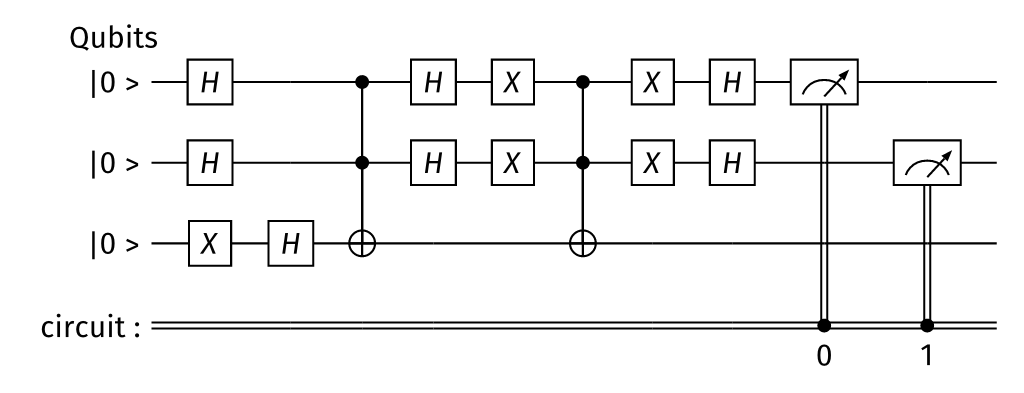
\includegraphics[width=0.9\textwidth]{images/basic-algorithms/3-qubits-grover.png}
    \caption{Grover-Algorithmus für $n=2$ (das gesuchte Element - $11$)}
    \label{fig:grover-three-bits}
\end{figure}

Zu Beginn, noch vor dem Start der Iterationen, müssen alle Qubits – einschließlich des Hilfsqubits – in eine Superposition gebracht werden. Dabei sollen sich zu Anfang alle Qubits im Zustand $0$ befinden, mit Ausnahme des Hilfsqubits, der vor der Hadamard-Operation in den Zustand $1$ gesetzt wird.\\

Nach Anwendung des Hadamard-Gatters befindet sich das Hilfsqubit somit im Zustand $\frac{1}{\sqrt{2}}(|0\rangle - |1\rangle)$, während alle übrigen Qubits den Zustand $\frac{1}{\sqrt{2}}(|0\rangle + |1\rangle)$ annehmen.

Anschließend beginnen die Iterationen. Jede Iteration besteht aus zwei Phasen. Die erste Phase ist die Anwendung der Orakelfunktion. Wie es in Grover-Algorithmus \ref{alg:grover} vorgestellt wurde, handelt es sich um eine Funktion, die effizient bestimmen kann, welcher Index dem gesuchten Element entspricht. Zwar kann diese Funktion den Index nicht direkt mitteilen, jedoch ist sie in der Lage, diesen Zustand mit einem Minuszeichen zu markieren.

Um das Funktionsprinzip des Algorithmus in diesem Beispiel besser zu verstehen, definieren wir eine vereinfachte Orakelfunktion manuell. Dabei ist zu beachten, dass die tatsächliche Orakelfunktion in der Praxis spezifisch an die jeweilige Aufgabe angepasst ist und daher möglicherweise anders implementiert wird. Auf die konkrete technische Realisierung der Orakelfunktion zur Datensuche gehen wir hier nicht ein, da dies den grundlegenden Ablauf von Grovers Algorithmus nicht beeinflusst.

Für das Verständnis des Grover-Algorithmus ist es entscheidend nachzuvollziehen, wie sich die Zustände der Qubits verändern, bis zum Zeitpunkt der Messung, die schließlich den gesuchten Index liefert.In diesem Beispiel haben wir als das gesuchte Index $11$ definiert - so wie es in dem Beispiel von Karten gab. Das bedeutet, dass die Messung am Ende genau dieses Ergebnis liefern soll. Wir modellieren daher ein Orakel, das genau diesen Index markiert. Als solche Orakelfunktion eignet sich das Toffoli-Gatter ($CCNOT$), das bei Ansteuerung beider Kontrollqubits mit dem Wert $1$ ein $X$-Gatter auf das Zielqubit – in diesem Fall das Hilfsqubit – anwendet:

\begin{definition}[Toffoli-Gatter]
\label{def:toffoli}
Das Toffoli-Gatter, auch bekannt als $CCNOT$-Gatter (für „controlled-controlled-not“), ist eine Erweiterung des bekannten $CNOT$-Gatters mit zwei Steuerbits und einem Zielbit. Das bedeutet: Das Zielbit (das dritte Bit) wird genau dann invertiert, wenn sowohl das erste als auch das zweite Steuerbit den Wert $1$ haben.(\cite{toffoli_proceedings_1980})
\end{definition}

Das Toffoli-Gatter sieht folgendermaßen aus:
\begin{figure}[H]
    \centering
    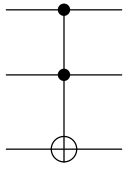
\includegraphics[width=0.2\textwidth]{images/basic-algorithms/toffoli.png}
    \caption{$CCNOT$ - Toffoli-Gatter}
    \label{fig:toffoli-gate}
\end{figure}

 Für die Zustände der oberen Qubits, die die Indizes $00$, $01$ und $10$ codieren, bleibt das Toffoli-Gatter ohne Wirkung – der Hilfsqubit verbleibt in dem Zustand $\frac{1}{\sqrt{2}}(|0\rangle - |1\rangle)$.\\

 Erst beim Index $11$ wird das Gatter aktiv: Es wendet das $X$-Gatter auf den Hilfsqubit an, wodurch dieser den Zustand $\frac{1}{\sqrt{2}}(|1\rangle - |0\rangle)$ annimmt \ref{def:toffoli}. Dieser lässt sich äquivalent als $-\frac{1}{\sqrt{2}}(|0\rangle - |1\rangle)$ schreiben – das Minuszeichen erscheint also vor dem gesamten Zustand.\\

 Dieses Minuszeichen bezieht sich nicht nur auf den Hilfsqubit, sondern auf den gesamten Zustand, der dem Index $11$ entspricht. Daher kann man den Hilfsqubit als unverändert betrachten und das Vorzeichen dem Zustand der oberen Qubits zuordnen. Damit ist der Index $11$ als der gesuchte Zustand mit einem Minus gekennzeichnet. Anders ausgedrückt: Die Orakelfunktion transformiert den Zustand $|11\rangle\,|q_{\text{3}}\rangle$ in $-|11\rangle\,|q_{\text{3}}\rangle$, wobei $|q_{\text{3}}\rangle$ den Zustand des Hilfsqubits bezeichnet.

Den Zustand des Quantensystems nach Anwendung des Orakels können wir folgendermaßen ausdrücken (der Hilfsqubit steht in der rechten Klammer):

$$
|\psi\rangle = \frac{1}{2\sqrt{2}} (|00\rangle + |01\rangle + |10\rangle - |11\rangle)(|0\rangle - |1\rangle)
$$

Damit ist der erste Teil der ersten Iteration abgeschlossen. Der gesuchte Index wurde markiert, aber eine sofortige Messung der Qubits würde keinen Nutzen bringen – das Minuszeichen zeigt sich im Messergebnis nicht. Außerdem würde der Index $11$ mit einer Wahrscheinlichkeit von nur $0{,}25$ erscheinen – genau wie alle anderen Indizes.

Um die weiteren Schritte besser zu verstehen, stellen wir uns die erste Hälfte des Algorithmus grafisch als Zustandsvektor vor. Die horizontale Achse definieren wir als Einheitsvektor, der alle Zustände der Superposition enthält – mit Ausnahme des gesuchten Zustands. Die vertikale Achse steht für den gesuchten Basiszustand.

Der Zustandsvektor $c$, also der Zustand des Systems vor der ersten Iteration, ist eine Linearkombination dieser beiden Basisvektoren entlang der horizontalen und vertikalen Achse.\ref{fig:initial-grover-three-qubits}

\begin{figure}[H]
    \centering
    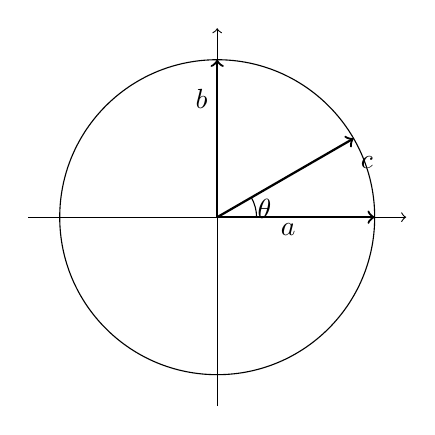
\begin{tikzpicture}[scale=2]
    % Draw coordinate axes
    \draw[->] (-1.2, 0) -- (1.2, 0); % x-axis
    \draw[->] (0, -1.2) -- (0, 1.2); % y-axis

    % Draw the unit circle
    \draw (0,0) circle(1);

    % Angle theta
    \draw[->, thick] (0,0) -- (0.866,0.5); % hypotenuse (c)
    \node at (0.95,0.35) {$c$};

    % Projection on x-axis (a)
    \draw[->, thick] (0,0) -- (1,0);
    \node at (0.45,-0.08) {$a$};

    % Projection on y-axis (b)
    \draw[->, thick] (0,0) -- (0,1);
    \node at (-0.1,0.75) {$b$};

    % Angle label θ
    \draw (0.25,0) arc[start angle=0,end angle=30,radius=0.25];
    \node at (0.3,0.05) {$\theta$};
\end{tikzpicture}
    \caption{Der initiale Zustand des Systems}
    \label{fig:initial-grover-three-qubits}
\end{figure}

Im Fall dieses Beispiels (ein System aus zwei Qubits mit dem gesuchten Index $11$) lässt sich der Zustandsvektor $c$ durch die Koordinaten $x$ und $y$ wie folgt darstellen:

$$
\frac{1}{2}(|00\rangle + |01\rangle + |10\rangle + |11\rangle) = x \cdot \frac{1}{\sqrt{3}}(|00\rangle + |01\rangle + |10\rangle) + y \cdot |11\rangle
$$

\noindent Aus dieser Gleichung ergibt sich: $x = \frac{\sqrt{3}}{2}$ und $y = \frac{1}{2}$.\\

Anhand dieser Koordinaten erkennt man, dass der Winkel $\theta$ zwischen dem Vektor $c$ und der horizontalen Achse gleich $\frac{\pi}{6}$ ist. Vorausblickend lässt sich sagen: Unser Ziel ist es, diesen Winkel auf $\frac{\pi}{2}$ (oder zumindest in dessen Nähe) zu bringen – also den Zustand nahezu vollständig in Richtung des gesuchten Basiszustands zu drehen, sodass bei der anschließenden Messung mit hoher Wahrscheinlichkeit das gewünschte Ergebnis erscheint.

Die Koordinaten des aktuellen Zustandsvektors lassen sich über den Winkel $\theta$ wie folgt beschreiben:

$$
x = \cos{\theta}
$$
$$
y = \sin{\theta}
$$

Zur Klarstellung: Der Hilfsqubit wird in der Kreisdarstellung nicht berücksichtigt, da er nicht zur Codierung des Index dient, sondern lediglich zur Markierung des gesuchten Zustands verwendet wird.

Nach Anwendung der Orakelfunktion spiegelt sich der Zustandsvektor an der horizontalen Achse. Dies liegt daran, dass seine vertikale Komponente (der Anteil des Vektors $|11\rangle$) negativ wird. Der resultierende Vektor $c_{1b}$ ist somit die Spiegelung des ursprünglichen Vektors $c$ um den Winkel $\theta$ nach unten relativ zur Horizontalen:

\begin{figure}[H]
    \centering
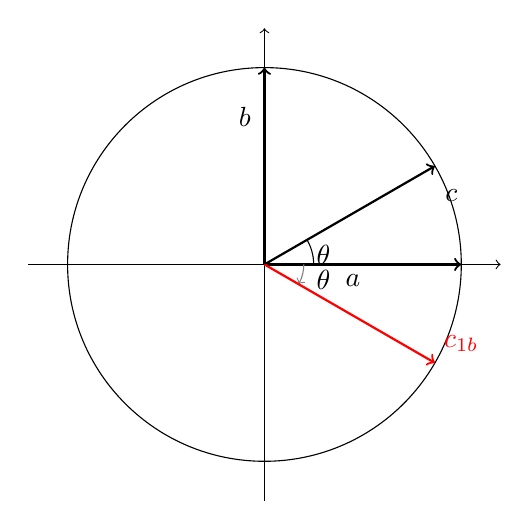
\begin{tikzpicture}[scale=2.5]

    % Draw coordinate axes
    \draw[->] (-1.2, 0) -- (1.2, 0); % x-axis
    \draw[->] (0, -1.2) -- (0, 1.2); % y-axis

    % Draw the unit circle
    \draw (0,0) circle(1);

    % Main vector c (black)
    \draw[->, thick] (0,0) -- (0.866,0.5);
    \node at (0.95,0.35) {$c$};

    % Projection on x-axis (a)
    \draw[->, thick] (0,0) -- (1,0);
    \node at (0.45,-0.08) {$a$};

    % Projection on y-axis (b)
    \draw[->, thick] (0,0) -- (0,1);
    \node at (-0.1,0.75) {$b$};

    % First angle theta
    \draw (0.25,0) arc[start angle=0,end angle=30,radius=0.25];
    \node at (0.3,0.05) {$\theta$};

    % Second angle theta (for red vector)
    \draw[gray, ->] (0.2,0) arc[start angle=0,end angle=-30,radius=0.2];
    \node at (0.3,-0.08) {$\theta$};

    % Red vector c_{1b}
    \draw[->, thick, red] (0,0) -- (0.866,-0.5);
    \node[red] at (1.0,-0.4) {$c_{1b}$};

\end{tikzpicture}
    \caption{Der Zustand des Systems nach der ersten Teil der erste Iteration}
    \label{fig:after-first-part-grover-three-qubits}
\end{figure}

Diese Spiegelung erfolgt in diesem Beispiel durch die Anwendung des $CCNOT$-Gatters. Allgemein jedoch lässt sich dieser Schritt der Orakelfunktion durch folgende Operation beschreiben:

$$
U_{1b} = I - 2|b\rangle \langle b|
$$

Hier steht $U_{1b}$ für die Orakelfunktion. Diese Operation kehrt ausschließlich das Vorzeichen der vertikalen Komponente des Zustandsvektors um, was genau zur beschriebenen Spiegelung führt.

Überprüfen wir nun die Wirkung dieser Formel anhand des Beispiels:

\begin{align*}
U_{1b} |c\rangle &= (I - 2|11\rangle \langle 11|) \cdot \frac{1}{2}(|00\rangle + |01\rangle + |10\rangle + |11\rangle) \\
&= \frac{1}{2} \left( |00\rangle + |01\rangle + |10\rangle + |11\rangle - 2|11\rangle \right) \\
&= \frac{1}{2} (|00\rangle + |01\rangle + |10\rangle - |11\rangle)
\end{align*}

Damit ist der erste Teil der Iteration abgeschlossen.

Nun wenden wir uns dem zweiten Teil der ersten Iteration zu. In diesem Schritt erfolgt eine weitere Spiegelung – jedoch nicht mehr an der horizontalen Achse, sondern am ursprünglichen Zustandsvektor $c$. Es lässt sich leicht erkennen, dass der neue Zustandsvektor danach dem Ausdruck

$$
\cos(3\theta)|a\rangle + \sin(3\theta)|b\rangle
$$

\noindent entspricht. Das bedeutet, der Winkel zwischen dem Vektor und der horizontalen Achse ist nun $3\theta$. Der Zustand wurde also weiter in Richtung des gesuchten Basiszustands $|b\rangle$ gedreht.

\begin{figure}[H]
    \centering
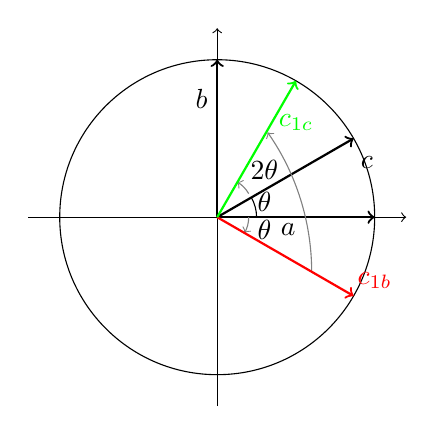
\begin{tikzpicture}[scale=2]

    % Draw coordinate axes
    \draw[->] (-1.2, 0) -- (1.2, 0); % x-axis
    \draw[->] (0, -1.2) -- (0, 1.2); % y-axis

    % Draw the unit circle
    \draw (0,0) circle(1);

    % Main vector c (black)
    \draw[->, thick] (0,0) -- (0.866,0.5);
    \node at (0.95,0.35) {$c$};

    % Projection on x-axis (a)
    \draw[->, thick] (0,0) -- (1,0);
    \node at (0.45,-0.08) {$a$};

    % Projection on y-axis (b)
    \draw[->, thick] (0,0) -- (0,1);
    \node at (-0.1,0.75) {$b$};

    % First angle theta
    \draw (0.25,0) arc[start angle=0,end angle=30,radius=0.25];
    \node at (0.3,0.1) {$\theta$};

    % Second angle theta (for red vector)
    \draw[gray, ->] (0.2,0) arc[start angle=0,end angle=-30,radius=0.2];
    \node at (0.3,-0.08) {$\theta$};

    % Third angle theta (for red vector)
    \draw[gray, ->] (0.2,0.15) arc[start angle=30,end angle=60,radius=0.2];
    \node at (0.3,0.3) {$2\theta$};

    \draw[gray, ->] (0.6,-0.35) arc[start angle=0,end angle=35,radius=1.55];

    % Red vector c_{1b}
    \draw[->, thick, red] (0,0) -- (0.866,-0.5);
    \node[red] at (1.0,-0.4) {$c_{1b}$};

    % Green vector c_{1c}
    \draw[->, thick, green] (0,0) -- (0.5,0.866);
    \node[green] at (0.5,0.6) {$c_{1c}$};

\end{tikzpicture}
    \caption{Der Zustand des Systems nach der zweiten Teil der erste Iteration}
    \label{fig:after-second-part-grover-three-qubits}
\end{figure}
Die Operation zur Erzeugung des reflektierten Vektors $c_{1c}$ sieht wie folgt aus:

$$
U_{1c} = 2|c\rangle \langle c| - I
$$

Berechnen wir den resultierenden Vektor $c_{1c}$ für unser Beispiel:

\begin{align*}
U_{1c} |c_{1b}\rangle &= \left(2|c\rangle \langle c| - I\right) \cdot \frac{1}{2} (|00\rangle + |01\rangle + |10\rangle - |11\rangle) \\
&= |11\rangle
\end{align*}

Es fand eine Spiegelung des Zustandsvektors $|c_{1b}\rangle$ an $|c\rangle$ statt. Wenn man den Vektor $|c_{1b}\rangle$ als Linearkombination $k_1 |c\rangle + k_2 |c_{\perp}\rangle$ schreiben kann, wobei $|c_{\perp}\rangle$ senkrecht auf $|c\rangle$ steht und $k_1$, $k_2$ reelle Koeffizienten sind, dann ergibt sich der gespiegelte Vektor zu:

$$
k_1 |c\rangle - k_2 |c_{\perp}\rangle
$$

Genau dies geschieht hier: Die Komponente entlang $|c\rangle$ bleibt erhalten, während die senkrechte Komponente ihr Vorzeichen ändert. In unserer Quantenschaltung wird dieser zweite Teil der Iteration folgendermaßen implementiert:

\begin{figure}[h!]
    \centering
    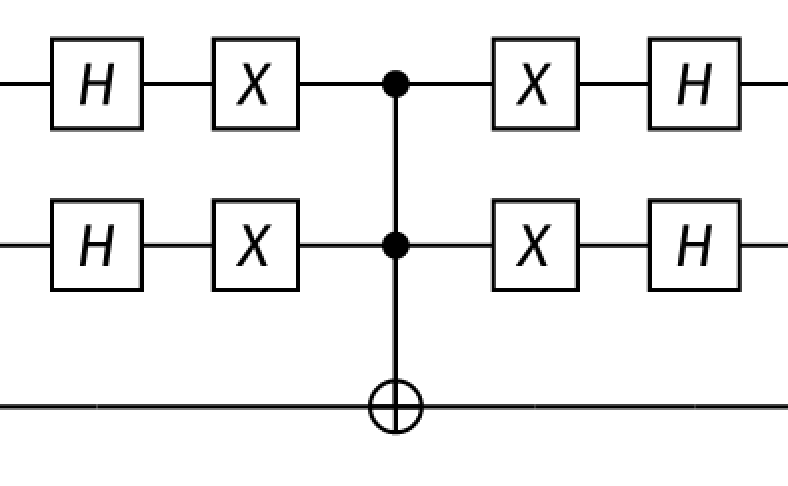
\includegraphics[width=0.4\textwidth]{images/basic-algorithms/grover-2-iteration.png}
    \caption{Zweite Iteration - $U_{1c}$}
    \label{fig:grover-second-iteration}
\end{figure}

Zunächst wird der Hadamard-Operator auf den ersten und zweiten Qubit angewendet. Dies vereinfacht unsere Aufgabe erheblich, da die Reflexion des Zustandsvektors nun nicht mehr relativ zum Superpositionszustand $\frac{1}{2}(|00\rangle + |01\rangle + |10\rangle + |11\rangle)$ erfolgen muss, sondern relativ zum Zustand $|00\rangle$.

Um die Spiegelung durchzuführen, müssten wir eigentlich allen Zuständen außer dem Nullzustand ein negatives Vorzeichen zuweisen. Stattdessen nutzen wir jedoch einen Trick: Wir versehen lediglich den Zustand $|00\rangle$ mit einem Minuszeichen und lassen alle übrigen Superpositionszustände unverändert. Dies erreichen wir durch eine gezielte Abfolge von Gattern: zuerst $X$-Gatter, dann ein $CCNOT$-Gatter, und danach wird die Transformation durch Umkehr der Schritte rückgängig gemacht – also erneut $X$-Gatter und anschließend Hadamard-Gatter.

Aufgrund dieses Tricks (Negation nur des Nullzustands) ergibt sich in unserem Beispiel mit zwei Qubits nicht $|11\rangle$, sondern $-|11\rangle$ als Ergebnis – abgesehen von einer globalen Phase. Dies ist jedoch unproblematisch, da sich die globale Phase beim Messen nicht auswirkt und wir den gesuchten Index trotzdem korrekt erhalten.

Aus der Darstellung auf dem Einheitskreis, die den Zustand des Systems nach der zweiten Hälfte der ersten Iteration veranschaulicht, wird deutlich, dass der Zustandsvektor mit jeder weiteren Iteration der Vertikalen näherkommt. In unserem konkreten Fall beträgt der Winkel zwischen Zustandsvektor und Horizontaler nach Abschluss der ersten Iteration bereits $3\theta$, was genau dem gewünschten Winkel $\frac{\pi}{2}$ entspricht.

Im allgemeinen Fall ergibt sich der Winkel nach $t$ Iterationen zu:

$$
(2t + 1)\theta \approx \frac{\pi}{2}
$$

Daraus lässt sich die erforderliche Anzahl an Iterationen für den Grover-Algorithmus bestimmen. Wenn $t$ groß ist und $K = 1$ (für $K > 1$ ist der Schluss analog), wird der Winkel $\theta$ sehr klein. Daher kann man $\theta$ durch $\sin{\theta}$ ersetzen, und es gilt näherungsweise:

$$
\theta \approx \sin{\theta} = \frac{1}{\sqrt{N}}
$$

Daraus folgt:

$$
(2t + 1) \cdot \frac{1}{\sqrt{N}} \approx \frac{\pi}{2}
$$

Wenn man die Eins im Term $(2t + 1)$ vernachlässigt (für große $t$ zulässig), erhält man:

$$
t \approx \frac{\pi \sqrt{N}}{4}
$$

Wie wir bereits gesehen haben, besteht jede Iteration aus zwei Schritten. Der erste Schritt ist die Reflexion nach unten an der Horizontalen. Der zweite Schritt ist die Reflexion nach oben an der ursprünglichen Richtung, also am Vektor $c$. Dabei wird der Zustandsvektor stets auf einen größeren Winkel nach oben reflektiert als der Winkel der vorherigen Spiegelung nach unten. Genau dadurch nähert sich der Vektor bei jeder Iteration schrittweise der Vertikalen.\\

Wir haben ein Beispiel für die Anwendung des Grover-Algorithmus betrachtet. Im nächsten Kapitel werden wir uns mit der Zeitkomplexität beschäftigen und erläutern, warum dieser Algorithmus trotz der Anzahl an Iterationen dennoch schneller ist als klassische Suchalgorithmen.


\subsection{Komplexitätsanalyse}
Der Grover‐Algorithmus durchsucht eine unstrukturierte Datenbank der Größe \(N\) mithilfe eines Quantenorakels in \(\Theta(N)\) Orakelaufrufen. Anders ausgedrückt: Während die klassische Vollsuche im Mittel \(\Theta(N)\) Prüfungen erfordert, reduziert Grover die Zahl der notwendigen Prüfungen auf etwa $\frac{\pi}{4}\,\sqrt{N}\ $ das heißt auf die Quadratwurzel der Datenbankgröße.

Aus Sicht der Komplexitätstheorie bezeichnet man die Eingangsgröße mit \(n\), so dass $N = 2^n$.
Die Laufzeit des Grover‐Algorithmus lässt sich daher durch  
$O\bigl(2^{n/2}\bigr)$ beschreiben. Obwohl dies gegenüber dem klassischen \(O(2^n)\) einen erheblichen quadratischen Gewinn darstellt, wächst der Algorithmus bei zunehmender Zahl der Suchbits weiterhin exponentiell.

Die untere Schranke aus der Arbeit von Bennett–Bernstein–Brassard–Vazirani (\cite{zotero-1212}) zeigt, dass kein Quantenalgorithmus im Black‐Box‐Modell mit weniger als  
\[
\Omega(\sqrt{N})
\]  
Orakelaufrufen auskommen kann.(\cite{zotero-1211}) Damit ist der Grover‐Algorithmus in diesem Modell asymptotisch optimal: Ohne zusätzliche Struktur in der Datenbank lässt sich kein suprakquadratischer (etwa exponentieller) Vorteil erzielen.  


\section{Klassifikation von Algorithmen nach Zeitkomplexität}

Im Rahmen der theoretischen Informatik werden Entscheidungsprobleme nach der zur Lösung benötigten Zeit in verschiedene Klassen eingeordnet. Dabei interessiert insbesondere, welche Probleme auf einem klassischen bzw. quantenmechanischen Modell in polynomieller Zeit lösbar sind, und wie sich diese Klassen zueinander verhalten.\\

Zunächst versteht man unter der Klasse \(\mathbf{P}\) jene Probleme, für die es deterministische Algorithmen gibt, die auf einem klassischen Computer in polynomieller Zeit laufen. Formal heißt das: Ein Problem liegt in \(\mathbf{P}\), wenn es einen Algorithmus gibt, dessen Laufzeit durch einen Polynomausdruck \(O(n^k)\) für eine feste Konstante \(k\) beschränkt ist, wobei \(n\) die Eingabegröße bezeichnet. Probleme aus \(\mathbf{P}\) gelten als praktisch effizient lösbar, sofern der Exponent \(k\) nicht zu groß wird.\\

Die Klasse \(\mathbf{NP}\) (nondeterministic polynomial time) umfasst diejenigen Entscheidungsprobleme, bei denen eine etwaige Lösung auf einem klassischen Computer in polynomieller Zeit verifizierbar ist, auch wenn ein deterministischer polynomieller Lösungsalgorithmus bislang unbekannt ist. Ein typisches Beispiel ist das Teilmengen-Summen-Problem: Legt man dem Algorithmus als „Zertifikat“ eine vermutete Teilmenge vor, so kann man in \(O(n)\) bzw. \(O(n\log n)\) Zeit nachprüfen, ob die Summe den Zielwert ergibt.\\

Innerhalb von \(\mathbf{NP}\) existieren die \(\mathbf{NP}\)-\emph{vollständigen} Probleme (\(\mathbf{NP}\)\emph{-complete}), die zu den schwierigsten \(\mathbf{NP}\)-Problemen zählen. Ein Problem \(L\) ist genau dann \(\mathbf{NP}\)-vollständig, wenn \(L\in\mathbf{NP}\) und jedes andere Problem aus \(\mathbf{NP}\) in polynomieller Zeit auf \(L\) reduziert werden kann. Die berühmte \textsc{Clique}-Frage oder das \textsc{3-SAT}-Problem sind klassische Vertreter dieser Klasse. Gelingt es, eines dieser Probleme in polynomieller Zeit zu lösen, so hätte man damit einen polynomiellen Algorithmus für alle \(\mathbf{NP}\)-Probleme.\\

Die Klasse der \(\mathbf{NP}\)-\emph{harten} Probleme (\(\mathbf{NP}\)\emph{-hard}) enthält solche Probleme, auf die sich beliebige \(\mathbf{NP}\)-Probleme in polynomieller Zeit reduzieren lassen. Im Gegensatz zu \(\mathbf{NP}\)-vollständigen Problemen müssen \(\mathbf{NP}\)-harte Probleme selbst nicht in \(\mathbf{NP}\) liegen und können etwa gar nicht entscheidbar sein oder nur in exponentieller Zeit verifizierbar sein.\\

Wenn man zusätzlich zur deterministischen Rechenmaschine Zufallsbits zulässt und die Wahrscheinlichkeit, die richtige Entscheidung zu treffen, für positive und negative Instanzen jeweils oberhalb eines festen Schwellwerts (typischerweise \(>1/2\)) liegt, definiert man die Klasse \(\mathbf{BPP}\) (bounded‑error probabilistic polynomial time). Probleme in \(\mathbf{BPP}\) lassen sich mit Monte‑Carlo‑Algorithmen in polynomieller Zeit mit beliebig kleiner Fehlerrate lösen.(\cite{zotero-1212}) \\

Der quantenmechanische Gegenpart zu \(\mathbf{BPP}\) ist die Klasse \(\mathbf{BQP}\) (bounded‑error quantum polynomial time).(\cite{zotero-1212}) Hierbei kann ein Quantenalgorithmus für ein Problem in polynomieller Zeit auf einem Quantencomputer mit hoher Wahrscheinlichkeit das korrekte Ergebnis liefern. Ein bekanntes Beispiel ist die Ganzzahlfaktorzerlegung großer Zahlen mittels Shor’s Algorithmus, der das hierfür klassische \(\mathbf{NP}\)-Problem in polynomieller Zeit auf einem Quantencomputer löst.

\begin{figure}[h]
  \centering
  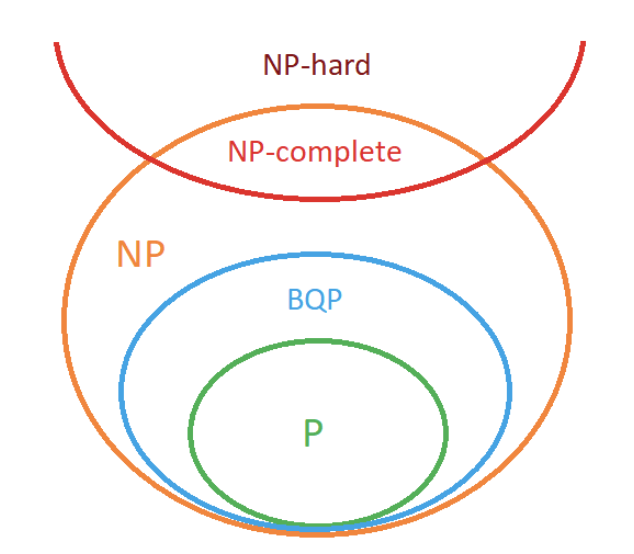
\includegraphics[width=0.7\textwidth]{images/basic-algorithms/problem-classes.png}
  \caption{Übersicht der wichtigsten Zeitkomplexitätsklassen: \(\mathbf{P}\subseteq \mathbf{BQP}\subseteq \mathbf{NP}\subseteq \mathbf{NP}\text{-hard}\) und die Lage von \(\mathbf{NP}\)-complete Problemen innerhalb von \(\mathbf{NP}\).}
  \label{fig:problem_classes}
\end{figure}

Abschließend lässt sich festhalten, dass die Frage, ob \(\mathbf{P}=\mathbf{NP}\) gilt, zu den bedeutendsten offenen Problemen der Informatik zählt. Auch der Vergleich zwischen klassischen und quantenmechanischen Modellen, speziell die Vermutung \(\mathbf{P}\subsetneq \mathbf{BQP}\subseteq \mathbf{NP}\), prägt die Forschung im Bereich effizienter Algorithmen maßgeblich.

\section{Quantum Safe Algorithmen}

\subsection*{Einleitung}

Mit der rasanten Entwicklung von Quantencomputern stehen klassische Verschlüsselungsverfahren vor einer existenziellen Bedrohung. Während heutige Systeme auf der Annahme beruhen, dass bestimmte mathematische Probleme schwer zu lösen sind, können Quantenalgorithmen wie \textit{Shor’s Algorithmus} oder \textit{Grover’s Algorithmus} diese Probleme effizient berechnen – und damit die Sicherheit brechen, auf die heutige digitale Kommunikation angewiesen ist.

Diese Bedrohung macht sogenannte \textbf{Quantum Safe Algorithmen} notwendig – kryptographische Verfahren, die auch gegen Angriffe durch leistungsfähige Quantencomputer resistent sind. Zwei Hauptansätze stehen im Zentrum der Forschung:

\begin{itemize}
  \item \textbf{Quantum Key Distribution (QKD)} – ein Verfahren, das physikalische Gesetze der Quantenmechanik nutzt, um absolut sichere Schlüsselverteilungen zu ermöglichen.
  \item \textbf{Post-Quantum Cryptography (PQC)} – klassische, quantenresistente Algorithmen, die auf heutigen Geräten ausgeführt werden können.
\end{itemize}

In diesem Kapitel werfen wir einen Blick auf beide Ansätze – und erläutern insbesondere die jüngsten Fortschritte durch das NIST (National Institute of Standards and Technology), das 2022 erste standardisierungsreife Algorithmen bekannt gegeben hat.

\subsection{Quantum Key Distribution}

Quantum Key Distribution (QKD) ermöglicht es, kryptografische Schlüssel über unsichere Kanäle zu übertragen – mit einem entscheidenden Vorteil: Jeder Abhörversuch verändert unweigerlich den Zustand der übertragenen Quanteninformation und kann somit erkannt werden.

Ein klassisches Beispiel für ein QKD-Protokoll ist das \textbf{BB84-Protokoll}, das 1984 von Bennett und Brassard entwickelt wurde und später, im Jahr 2000, von Peter W. Shor and John Preskill geprüft wurde. Es nutzt die Polarisation von Photonen, um binäre Informationen zu codieren. Der Ablauf besteht aus drei Phasen:

\begin{itemize}
  \item \textbf{Key Exchange:} Alice sendet zufällig polarisierte Photonen an Bob, der sie in zufällig gewählten Basen misst.
  \item \textbf{Key Sifting:} Über einen klassischen Kanal gleichen beide ihre verwendeten Basen ab und behalten nur die Werte, bei denen die Basen übereinstimmten.
  \item \textbf{Key Distillation:} Durch Stichproben wird geprüft, ob Abhörversuche stattfanden. Die finale Schlüssellänge ergibt sich nach dieser Bereinigung.
\end{itemize}

\noindent Neben BB84 existieren weitere bedeutende Protokolle:

\begin{itemize}
  \item \textbf{B92} (reduzierte Variante mit zwei Zuständen)
  \item \textbf{E91} (nutzte erstmals Quantenverschränkung)
  \item \textbf{BBM92}, \textbf{SARG04}, \textbf{DPS}, \textbf{COW}, \textbf{GG02} (verschiedene Weiterentwicklungen)
\end{itemize}

Für eine detaillierte Übersicht der Protokolle und deren Unterschiede siehe das Paper:
\textit{An Overview of Quantum-Safe Approaches: Quantum Key Distribution and Post-Quantum Cryptography} von Guobin Xu et al.

\subsection{Post-Quantum Cryptographie Algorithmen}

Da QKD mit hohen technischen und infrastrukturellen Anforderungen verbunden ist, setzt sich in der Praxis vor allem die \textbf{Post-Quantum Cryptography (PQC)} durch. Sie nutzt klassische Rechenverfahren, basiert jedoch auf mathematischen Problemen, die auch für Quantencomputer als schwierig gelten.

Das US-amerikanische \textbf{NIST} hat im Rahmen eines mehrjährigen Wettbewerbs Verfahren für zwei Hauptkategorien gesucht:

\begin{itemize}
  \item \textbf{Public-Key Encryption and Key Establishment (KEM)}
  \item \textbf{Digitale Signaturverfahren}
\end{itemize}

\noindent Nach mehreren Runden wählte NIST im Juli 2022 vier Algorithmen aus, die als erste Quantum Safe Standards empfohlen werden.

\noindent Für Verschlüsselung und Schlüsselaustausch nominierte NIST:

\begin{itemize}
  \item \textbf{CRYSTALS-Kyber} – 2017, J. Bos et al.
\end{itemize}

\vspace{0.5em} % optionaler vertikaler Abstand

\noindent Für digitale Signaturen nominierte NIST:

\begin{itemize}
  \item \textbf{CRYSTALS-Dilithium} – 2018, L. Ducas et al.

  \item \textbf{Falcon} – 2018, P.-A. Fouque et al.

  \item \textbf{SPHINCS+} – 2019, D. J. Bernstein et al.
\end{itemize}

\subsubsection*{CRYSTALS-Kyber}

\textbf{CRYSTALS-Kyber} ist ein \textit{lattice-basiertes Key Encapsulation Mechanism (KEM)}. Es basiert auf dem sogenannten \textit{Module Learning with Errors (MLWE)}-Problem, das auch von Quantencomputern bislang nicht effizient gelöst werden kann.

Der Algorithmus nutzt Polynomarithmetik und besteht aus drei Hauptschritten:

\begin{enumerate}
  \item \textbf{Schlüsselerzeugung:} Öffentlicher und privater Schlüssel werden erzeugt.
  \item \textbf{Encapsulation:} Ein gemeinsamer Schlüssel wird erzeugt und verschlüsselt übertragen.
  \item \textbf{Decapsulation:} Der Empfänger entschlüsselt den Schlüssel mit seinem privaten Schlüssel.
\end{enumerate}

\noindent Kyber bietet drei Sicherheitsniveaus, die sich durch unterschiedliche Parametergrößen unterscheiden und an klassische AES-Sicherheitsstufen angelehnt sind:

\begin{itemize}
  \item \textbf{Kyber-512} – Sicherheitsniveau 1 (vergleichbar mit AES-128)
  \item \textbf{Kyber-768} – Sicherheitsniveau 3 (vergleichbar mit AES-192)
  \item \textbf{Kyber-1024} – Sicherheitsniveau 5 (vergleichbar mit AES-256)
\end{itemize}

\subsubsection*{CRYSTALS-Dilithium}

\textbf{CRYSTALS-Dilithium} ist ein digitaler Signaturalgorithmus, ebenfalls basierend auf \textit{MLWE} und \textit{MSIS} (Module Short Integer Solution). Die Signaturerzeugung verwendet die \textit{Fiat-Shamir-Transformation}, die aus einem interaktiven Zero-Knowledge-Protokoll eine nicht-interaktive Signatur macht.

Dilithium bietet drei Sicherheitsniveaus:

\begin{itemize}
  \item \textbf{Dilithium2}
  \item \textbf{Dilithium3}
  \item \textbf{Dilithium5}
\end{itemize}

Die Vorteile liegen in der schnellen Verifikation, der Robustheit gegen Seitenkanalangriffe und der guten Performance. Diese Eigenschaften machen Dilithium zu einem führenden Kandidaten im Bereich der quantensicheren digitalen Signaturen.
\printbibliography